
%
% Original author:
% Frits Wenneker (http://www.howtotex.com) with extensive modifications by
% Vel (vel@LaTeXTemplates.com)
%
% License:
% CC BY-NC-SA 3.0 (http://creativecommons.org/licenses/by-nc-sa/3.0/)
%
%%%%%%%%%%%%%%%%%%%%%%%%%%%%%%%%%%%%%%%%%
\documentclass[twoside,twocolumn]{article}

%\usepackage{listings}
\usepackage[utf8]{inputenc}
\usepackage{amsmath}
\usepackage{algorithm}
\usepackage{standalone}
\usepackage{algpseudocode}
\usepackage[backend=bibtex8,style=authoryear]{biblatex}
\bibliography{citations}

\usepackage[sc]{mathpazo} % Use the Palatino font
\usepackage[T1]{fontenc} % Use 8-bit encoding that has 256 glyphs
\linespread{1.05} % Line spacing - Palatino needs more space between lines
\usepackage{microtype} % Slightly tweak font spacing for aesthetics
\usepackage{graphicx}
\usepackage[dutch]{babel} % Language hyphenation and typographical rules

\usepackage[hmarginratio=1:1,top=32mm,columnsep=20pt]{geometry} % Document margins
\usepackage[hang, small,labelfont=bf,up,textfont=it,up]{caption} % Custom captions under/above floats in tables or figures
\usepackage{booktabs} % Horizontal rules in tables

\usepackage{lettrine} % The lettrine is the first enlarged letter at the beginning of the text

\usepackage{enumitem} % Customized lists
\setlist[itemize]{noitemsep} % Make itemize lists more compact

\usepackage{abstract} % Allows abstract customization
\renewcommand{\abstractnamefont}{\normalfont\bfseries} % Set the "Abstract" text to bold
\renewcommand{\abstracttextfont}{\normalfont\small\itshape} % Set the abstract itself to small italic text

\usepackage{titlesec} % Allows customization of titles
\renewcommand\thesection{\Roman{section}} % Roman numerals for the sections
\renewcommand\thesubsection{\roman{subsection}} % roman numerals for subsections
\renewcommand\thesubsubsection{\arabic{subsubsection}}
\titleformat{\section}[block]{\large\scshape\centering}{\thesection.}{1em}{} % Change the look of the section titles
\titleformat{\subsection}[block]{\large}{\thesubsection.}{1em}{} % Change the look of the section titles
\titleformat{\subsubsection}[block]{\normalsize}{\thesubsubsection.}{1em}{}
\setlength{\parindent}{0cm}
\usepackage{fancyhdr} % Headers and footers
\pagestyle{fancy} % All pages have headers and footers
\fancyhead{} % Blank out the default header
\fancyfoot{} % Blank out the default footer
\fancyhead[C]{ Tobiah Lissens $\bullet$ December 2017 $\bullet$ Huffman Algoritmen} % Custom header text
\fancyfoot[RO,LE]{\thepage} % Custom footer text

\usepackage{titling} % Customizing the title section

\usepackage{hyperref} % For hyperlinks in the PDF
%\usepackage[all]{hypcap}
\usepackage{tikz} % For drawing graphs
\usepackage{array}
\usepackage[figurename=Figuur]{caption}
\usetikzlibrary{
  shapes.multipart,
  matrix,
  positioning,
  shapes.callouts,
  shapes.arrows,
  calc,
  graphs,
  }
\floatname{algorithm}{Algoritme}
%\renewcommand{\algorithmcfname}{Algoritme}

%----------------------------------------------------------------------------------------
%	TITLE SECTION
%----------------------------------------------------------------------------------------

\setlength{\droptitle}{-4\baselineskip} % Move the title up

\pretitle{\begin{center}\Huge} % Article title formatting
\posttitle{\end{center}} % Article title closing formatting
\title{Algoritmen en datastructuren 3 \\ Huffman algoritmen } % Article title
\author{%
\textsc{Tobiah lissens}\\[1ex]% Your name
\normalsize Universiteit Gent \\ % Your institution
}
\date{6 December 2017} % Leave empty to omit a date

\renewcommand{\maketitlehookd}{%
\renewcommand{\abstractname}{Samenvatting}
\begin{abstract}
\noindent In dit verslag worden verschillende Huffman algoritmen besproken. 
Hierbij worden eerst enkele implemenatie details voor alle algoritmen besproken.
Verder worden enkele resultaten over de snelheid- en compressie-prestaties van alle algoritmes gegeven. Ook worden voorbeelden gegeven waarbij bepaalde algoritmen beter zullen presteren als andere. Algemeen kan geconcludeerd worden dat het standaard Huffman in de meeste gevallen de beste keuze is behalve wanneer de compressie op een online manier moet gebeuren of er veel lokaliteit in de tekst uit te buiten valt. Hiervoor kan via bloksgewijs standaard Huffman een oplossing voor geboden worden. 
\end{abstract}
}

%----------------------------------------------------------------------------------------

\begin{document}

\maketitle

%----------------------------------------------------------------------------------------
%	ARTICLE CONTENTS
%----------------------------------------------------------------------------------------

\section{Inleiding}
%zever
Compressie speelt vandaag de dag nog steeds een grote rol in de informatica.
Hierbij bestaat het probleem eruit een bepaald bestand op een zo'n klein mogelijk ander bestand af te beelden.
Dit is van toepassing bij bijvoorbeeld streaming sites zoals Youtube of Netflix.
Het Huffman algoritme is een van de vele mogelijke gekende compressie algoritmes. 
Dit verslag geeft een overzicht van enkele verschillende Huffman varianten en de implementaties hiervan. Verder worden ook enkele suggesties gegeven wanneer het een goed idee is een gegeven variant te gebruiken en wanneer deze te vermijden.

%----------------------------------------------------------------------------------------
\section{Enkele Algemene opmerkingen}
    \subsection{Diepte boom theorie vs praktijk}
        In theorie kan de Huffmanboom als we per byte encoderen een diepte van 254 bereiken.
        Indien er een extra nog niet gezien top\footnote{Verder wordt dit afgekort met nng.} aanwezig is zal de diepte ten hoogste 255 worden. Meer algemeen kunnen we dus stellen dat met een alfabet van grootte $n$, de diepte van de boom maximaal $n - 1$ zal zijn. De slechtste boom met een alfabet van grootte 3 wordt getoond in Figuur \ref{boom1}. 
    \begin{figure}[H]
        \begin{center}
        
            \begin{tikzpicture}
                [scale=.8, every node/.style={circle, draw}]
                \node (n1) at (1, 2) {4};
                \node (n2) at (0, 1) {2};
                \node (n3) at (2, 1) {2};
                \node (n4) at (1, 0) {1};
                \node (n5) at (3, 0) {1};
                
                \foreach \from\to in {n1/n2,n1/n3,n3/n4,n3/n5}
                    \draw (\from) -- (\to);
                
            \end{tikzpicture} 
        \end{center}
        \caption{Slechtste Huffmanboom}
        \label{boom1}
    \end{figure}    
    De kleinst mogelijke manier om een gelijkaardige boom op te stellen bekomt men wanneer de frequentietabel de Fibonacci reeks volgt. Als gevolg hiervan zal de grootte van bestanden die deze reeks volgen zeer groot worden. Het aantal bytes bij een Huffmanboom met diepte 64 is gelijk aan
    $\sum_{i=1}^{64} fib(i) = 15.61TiB $.
    Hieruit volgt dat in de praktijk padlengtes langer dan 64 zelden tot niet voorkomen en we het pad kunnen bij houden in een unsigned long long variable.
    
    \subsection{Encodeer algoritme}
     Het encoderen van een karakter\footnote{karakter en byte worden vaak door elkaar gebruikt hiermee bedoelen we 8 bits} kan op een eenvoudig manier gedaan worden. Indien er met een nng top\footnote{Dit is nodig voor adaptieve huffmanencodering.} wenst gewerkt te worden kan dit algoritme 
     eenvoudig aangepast worden. 
        \begin{algorithm}
            \begin{algorithmic}[1]
                \Procedure{encodeer}{\textit{tree}, \textit{c}}
                    \State \textit{stack} $\gets$ maak lege stack
                    \State \textit{top} $\gets$ getleaf(\textit{c})
                    \While{\textit{top} != root(\textit{tree})}
                    \If{left(parent(\textit{top})) == top}
                    \State push(\textit{stack},\textit{0})
                    \Else
                    \State push(\textit{stack},\textit{1})
                    \EndIf
                    \State top $\gets$ parent(\textit{top})
                    \EndWhile
                    \While {not empty(\textit{stack})}
                    \State print(pop(\textit{stack}))
                    \EndWhile
                \EndProcedure
            \end{algorithmic}
            \caption{Algemeen encodeer algoritme}
                        \label{alg:decodeer}

        \end{algorithm}
    
    \subsection{Decodeer Algoritme}
    Ook voor decoderen is slechts een eenvoudig algoritme vereist.
    Mits opnieuw enkele kleine aanpassingen kan dit werken met de nng top.
        \begin{algorithm}
            \caption{Algemeen encodeer algoritme}
            \begin{algorithmic}[1]
                \Procedure{Decodeer}{\textit{tree}}
                    \State \textit{top} $\gets$ root(tree) 
                    \While{not isleaf(\textit{top})}
                    \If{read\_bit() == 0}
                    \State top $\gets$ left(top)
                    \Else
                    \State top $\gets$ right(top)
                    \EndIf
                    \EndWhile
                    \State \Return value(\textit{top})
                \EndProcedure
            \end{algorithmic}
            \label{alg:encodeer}
        \end{algorithm}
    
    \subsection{Optimalisatie codeer- en decodeer Algoritmen}
        Zoals er in de 2 bovenstaande algoritmes wordt gedemonstreerd, moet het hele pad van de 
        wortel naar een blad doorlopen worden.
        Het zou dus voordelig zijn als de paden gecached of verkort kunnen worden. Hierdoor zou de 
        executie drastisch versneld kunnen worden.
        Jammergenoeg zal de adaptieve karakteristiek van vele gebruikte Huffman algoritmes dit verhinderen.
    
\section{Standaard Huffman}
    
    \subsection{Implementatie}
    % 2 queue's
    %cache padlenghts encoding 
    %fancy structure decoding
        \subsubsection{Encoderen}
          Een van de belangrijkste onderdelen bij standaard Huffman is het opbouwen van een boom.
          Dit kunnen we eenvoudig met het volgende algoritme doen:
          
            \begin{algorithm}
                \begin{algorithmic}[1]
                    \Procedure{bouw\_boom}{\textit{bladeren}}
                        \State \textit{queue1} $\gets$ sorteer(\textit{bladeren})
                        \State \textit{queue2} $\gets \textit{lege lijst}$
                        \While{size(\textit{queue1}) + size(\textit{queue2}) > 1}
                        \State \textit{first} $\gets$ poplowest(\textit{queue1}, \textit{queue2}) 
                        \State \textit{second} $\gets$ poplowest(\textit{queue1}, \textit{queue2})
                        \State \textit{parent} $\gets$ merge(\textit{first}, \textit{second})
                        \State enqueue(\textit{queue2}, \textit{parent})
                        \EndWhile
                        \State
                        \State \Return \textit{queue2}[0]
                    \EndProcedure
                \end{algorithmic}
                \caption{Standaard Huffman}
                \label{alg:bouwboom}
            \end{algorithm}
        
            Verder kunnen we bij standaard Huffman de paden ook cachen.
            Dit is mogelijk aangezien de paden van toppen naar bladeren niet worden aangepast tijdens het verloop van het encoderen.
            Door het cachen van paden kunnen we een karakter in $\Theta(1)$ encoderen in de plaats van $\Theta(d)$ met $d$ de lengte van het pad van de wortel naar het blad.
            Dit kan natuurlijk enkel op voorwaarde dat we het pad ook in constante tijd kunnen uitschrijven.
        \subsubsection{Decoderen} 
        %TODO start here
            Ook bij decoderen is eenvoudige optimalisatie mogelijk.
            Hierbij kan een normale Huffmanboom omgevormd worden naar een boom die meerdere bits per keer kan evalueren. 
            Stel we hebben de volgende boom in Figuur \ref{boom2} waarbij in de toppen aangeduid staat of ze het linkerkind of rechterkind zijn. 
            \begin{figure}[H]
                \begin{center}
                    \begin{tikzpicture}[scale=0.5,mynode/.style={circle, draw}]
                        \node[mynode] (n1) at (6, 5) {x};
                        \node[mynode] (n2) at (2, 4) {0};
                        \node[mynode] (n3) at (10, 4) {1};
                        \node[mynode] (n4) at (8, 2) {0};
                        \node[mynode,label=below:f] (n5) at (12, 2) {1};
                        \node[mynode, label=below:a] (n6) at (0, 2) {0};
                        \node[mynode] (n7) at (4, 2) {1};
                        \node[mynode, label=below:b] (n8) at (3, 0) {0};
                        \node[mynode, label=below:c] (n9) at (5, 0) {1};
                        \node[mynode, label=below:d] (n10) at (7, 0) {0};
                        \node[mynode,label=below:e] (n11) at (9, 0) {1};

                        \foreach \from\to in {n1/n3,n3/n5,n4/n11,n2/n7,n7/n9}
                            \draw (\from) -- (\to) ;node[midway,anchor=south]{1}; 
                        \foreach \from\to in {n3/n4,n4/n10,n1/n2,n2/n6, n7/n8}
                            \draw (\from) -- (\to);
                    \end{tikzpicture} 
                \end{center}
                \caption{Decodeer graaf}
                \label{decodeer-boom-simpel}

                \label{boom2}
            \end{figure}
            Een alternatieve voorstelling van dezelfde boom is afgebeeld in Figuur \ref{decodeer-boom-moeilijk}.
            \begin{figure}[H]
               
\documentclass[12pt,letterpaper]{article}

\usepackage[T1]{fontenc}
\usepackage{ae,aecompl}
\usepackage[utf8]{inputenc}
\usepackage{lmodern}
\usepackage{tikz}
\usetikzlibrary{shapes.multipart}

\begin{document}

  \begin{center}
    \begin{tikzpicture}[
      grow=right,
      level 1/.style={sibling distance=3cm,level distance=2.5cm},
      level 2/.style={sibling distance=1.5cm,level distance=2cm},
     % edge from parent/.style={draw=none},
      pointer/.style={thick, shorten >=5pt, ->,draw},
      dpointer/.style={draw},
      edge from parent/.style={draw=none},
      every label/.style={font=\footnotesize,draw=none},
      tree/.style={rectangle ,draw, text ragged, inner sep=2mm,minimum width=5mm},
      leaf/.style={circle, draw, inner sep=1mm,minimum width=5mm}
      ]


      \node[tree,label={$d=2$},rectangle split, rectangle split parts=4] (directory) {
        \nodepart{one} 00
        \nodepart{two} 01
        \nodepart{three} 10
        \nodepart{four} 11
      }
        child {
            node[leaf] (firstnode) {f,2}
        }
        child {
            node [tree, rectangle split, rectangle split parts=4](firsttree){
                \nodepart{one} 00
                \nodepart{two} 01
                \nodepart{three} 10
                \nodepart{four} 11
            }child{
                node[leaf] (firstfirstnode) {e,3}
            }
            child{
                node[leaf] (firstsecondnode) {d,3}
            };
        }
        child {
            node [tree, rectangle split, rectangle split parts=4](secondtree){
                \nodepart{one} 00
                \nodepart{two} 01
                \nodepart{three} 10
                \nodepart{four} 11
            }child{
                node[leaf] (secondfirstnode) {c,3}
            }
            child{
                node[leaf] (secondsecondnode) {b,3}
            };
        }
        child {
            node[leaf](lastnode) {a,2}
        };

      %level one edges
      \path(directory.four east) edge (firstnode);
      \path(directory.three east) edge (firsttree);
      \path(directory.two east) edge (secondtree);
      \path(directory.one east) edge (lastnode);
      
      %level two edges
      \path(firsttree.four east) edge (firstfirstnode);
      \path(firsttree.three east) edge (firstfirstnode);
      \path(firsttree.two east) edge (firstsecondnode);
      \path(firsttree.one east) edge (firstsecondnode);
      
      \path(secondtree.four east) edge (secondfirstnode);
      \path(secondtree.three east) edge (secondfirstnode);
      \path(secondtree.two east) edge (secondsecondnode);
      \path(secondtree.one east) edge (secondsecondnode);
    \end{tikzpicture}
  \end{center}

\end{document}

               \caption{Decodeer boom 2}
               \label{decodeer-boom-moeilijk}
            \end{figure}
            Het idee is om de paden van de boom zo kort mogelijk te houden en zo vaak mogelijk in constante tijd te kunnen decoderen.
            Dit kunnen we doen door de paden als index in een array te gebruiken.
            Indien het pad korter is dan $d$ met $2^d$ de lengte van de array dan wordt er met
            nullen aangvuld. Verder wordt er ook een pointer naar een blad voorzien waarbij de lengte van
             het pad wordt opgeslagen samen met het karakter dat hoort bij dit pad.
            Indien het pad langer is dan $d$ dan wordt er een pointer opgeslagen naar een nieuwe array met dezelfde eigenschappen. 
            In het bovenstaande voorbeeld is $d=2$, maar deze $d$ zal normaal gelijk zijn   
            aan 8. Hierdoor kunnen we per byte de boom indexeren.
    \subsection{Goede compressie}
    %Het beste geval bij standaard huffman bestaat uit een file met 1 of 2 karakters Dit valt ma
    % file met 1 of 2 karakters
    % file met 2 karkaters zal beter zijn dan alle andere varianten
    % bv aaaaaaaaaaaaaaaaaaaaaaaaaaaaaa
    % bv ababababababababababababababab (andere algoritmes hebben plaats voor nng nodig)
    Het beste geval bij standaard Huffman is een lang bestand waarbij er enkel gebruik wordt gemaakt van 1 of 2 verschillende karakters. Hierbij zal de boom dan altijd een diepte van 1 hebben. Hoe langer het bestand is hoe minder de initiële kost van het meesturen van de boom uit zal maken. Algemener kunnen we zeggen dat als een bestand weinig karakters bevat die veel herhaald worden het bestand zeer goed zal comprimeren.

%----------------------------------------------------------------------------------------
\section{Adaptive Huffman (FGK)}
    
    \subsection{Implementatie}
        Bij adaptieve Huffman is de grootste uitdaging een manier te vinden om de boom op een efficiente wijze up te daten. 
        Hiervoor is een simpel algoritme gegeven in \cite{cursusAD3}. 
        %\TODO citiation needed
        Bij dit algoritme zijn er echter nog 2 belangrijke opmerkingen te maken.
        De 1ste is het gebruik van slimme ordenummers. De 2de is op een efficiente manier 
        de volgende top te zoeken in een blok
        \footnote{Toppen behoren tot eenzelfde blok wanneer deze het zelfde gewicht hebben.}.
        \subsubsection{Ordenummers}
             In \cite{cursusAD3} krijgt de wortel het hoogste ordenummer. Dit is bij de implementatie echter
             zeer onhandig.
             Hierdoor zou bij het toevoegen van een nieuwe top de hele boom moeten 
             doorlopen worden en zou bij elk ordenummer + 2 moeten opgeteld worden.
             Een oplossing hiervoor bestaat uit de wortel het kleinste ordenummer te geven. Zijn 
             kinderen krijgen dan de ordenummers 1 en 2 etc.
             Hierdoor moeten er per toevoeging van een top maar 3 ordenummers worden aangepast 
             in de plaats van al de ordenummers in de boom.


        \subsubsection{Zoek de volgende top}
            Hier bestaat het probleem uit de top te zoeken die hetzelfde gewicht heeft, maar waarbij het ordenummer minimaal is. 
            In \cite{knuth85} wordt een oplossing geboden in constante tijd. % citation needed.
            Alhoewel deze methode in constante tijd gebeurt, is er wel een redelijk grote
            constante en complexe boekhouding voor nodig.
            Daarom is hier voor een andere oplossing gekozen. Deze is in theorie niet constant,
            maar in praktijk zal hij toch vaak zeer snel en bijna altijd constant zijn.
            
            \begin{algorithm}
                \begin{algorithmic}[1]
                    \Procedure{zoek\_volgende}{\textit{t}, \textit{map}}
                        \State \textit{t'} $\gets$ \textit{t}
                        \While{ord(\textit{t'}) != 0 and  weight(\textit{t}) == weight(map[ord(\textit{t'}) - 1)]}
                        \State t' $\gets$ map[ord(\textit{t'}) - 1]
                        \EndWhile 
                        \State \Return t'
                    \EndProcedure
                \end{algorithmic}
                \caption{Standaard Huffman}
                \label{alg:zoekvolgende}

            \end{algorithm}
            
    \subsection{Goede compressie}
    Het beste geval bij adaptive Huffman is gelijk aan dat van standaard Huffman. Alleen mag het bestand maar een herhaling van 1 karakter bevatten in de plaats van 2 karakters. Dit is omdat we hier rekening moeten houden met de nng top die bij adaptive Huffman ook altijd in de boom zal zitten.
    % file met 1 karakter niet met 2

%----------------------------------------------------------------------------------------
\section{Adaptieve Huffman met sliding window}

    \subsection{Implementatie}
        Het sliding window algoritme is zeer gelijkaardig aan het gewone adaptieve algoritme.
     Het grote verschil is dat enkel de laatste $n$ karakters in de boom worden gehouden. 
        Als gevolg hiervan wordt een additionele methode gebruikt die de frequentie van een bepaald blad vermindert met 1 en de boom dus ook terug transformeert zodat deze een geldige Huffmanboom blijft.
        Het algoritme dat de frequentie met 1 naar beneden haalt, is hier te vinden Algoritme \ref{alg:verlaagfrequentie}.
        \begin{algorithm}
            \begin{algorithmic}[1]
                \Procedure{verlaag\_frequentie}{\textit{c}}
                    \State \textit{t} $\gets$ top van \textit{c}
                    \While{\textit{t} != wortel}
                        \State \textit{t'} = lowest\_block(t)
                        \State swap(t, t')
                        \State lower\_weight(\textit{t})
                        \State \textit{t} = parent(t)
                    
                    \EndWhile
                    \State lower\_weight(t)
                    \State \If{weight(top van \textit{c}) == 0}
                        \State remove(top van \textit{c})
                    \EndIf
                \EndProcedure
            \end{algorithmic}
            \caption{Standaard Huffman}
            \label{alg:verlaagfrequentie}

        \end{algorithm}
        
        \subsubsection{Zoek vorige top}
        De zoek\_vorige functie is zeer gelijkaardig aan de zoek\_volgende \ref{alg:zoekvolgende} functie in de update methode.
        Het enige verschil met de zoek\_volgende in de update methode is dat nu het grootste ordernummer met het zelfde gewicht gezocht wordt in plaats van het kleinste.
        
        \subsubsection{Remove}
        De remove operatie bij sliding Huffman lijkt bedrieglijk gemakkelijk te zijn.
        Er is hier echter een addertje onder het gras.
        Stel je hebt de boom uit Figuur \ref{boom4} waarbij in elke top het ordenummer eerst staat, gevolgd door het gewicht. 
        \begin{figure}[H]
            \begin{center}
                \begin{tikzpicture}[every node/.style={circle, draw}]
                    \node (n1) {0,3}
                        child{
                            node[label=below:a] (n2) {2,1}
                        }
                        child{
                            node (n3) {1,2}
                                child{
                                    node [label=below:b] (n4) {3,1}
                                }
                                child{
                                    node (n5) {4,1}
                                        child {
                                            node [label=below:nng](n6) {6,0}
                                        }
                                        child{
                                            node [label=below:c] (n7) {5,1}
                                        }
                                }
                        };
                \end{tikzpicture}
            \end{center}
            \caption{Voorbeeld boom}
            \label{boom4}
        \end{figure}
        
        
        \begin{figure}[H]
            \begin{center}
                \begin{tikzpicture}[every node/.style={circle, draw}]
                    \node[label=above:verlaag c] (t1) {0,2}
                        child{
                            node[label=below:a] (t2) {2,1}
                        }
                        child{
                            node (t3) {1,2}
                                child{
                                    node[label=below:b] (t4) {3,1}
                                }
                                child{
                                    node[label=below:nng] (t5) {4,0}
                                }
                        };
                \end{tikzpicture} 
                \begin{tikzpicture}[every node/.style={circle, draw}]
                    \node[label=above:verhoog b] (n1) {0,2}
                        child{
                            node[label=below:a] (n2) {2,1}
                        }
                        child{
                            node (n3) {1,2}
                                child{
                                    node[label=below:{b}] (n4) {3,2}
                                }
                                child{
                                    node[label=below:nng] (n5) {4,0}
                                }
                        };    
                \end{tikzpicture}
        \end{center}
        \caption{Verwijder verkeerd}
        \label{fig:verwijderverkeerd}
    \end{figure}
    
    Bij het verhogen van de frequentie bij de boom afgebeeld in Figuur \ref{fig:verwijderverkeerd}, krijgen we een nieuwe boom die niet meer aan de voorwaarde van een Huffmanboom voldoet. Dit komt omdat we in de update operatie ervan uitgaan dat er een top met gewicht 0 in de boom zit.
    Hierdoor slaan we als het ware de swap met de parent over, deze is in dit geval echter niet legaal.
    Om de downdate compatibel met de update te houden moeten we in de remove dus een extra wissel invoeren en ervoor zorgen dat de ordenummers van nng, zijn broer en de parent altijd de hoogste 3 zijn.
    De correcte downdate is gedemonstreerd in Figuur \ref{nogboompjes}. 
    
    \begin{figure}[t]
        \begin{center}
            \begin{tikzpicture}[every node/.style={circle, draw}]
                \node[label=above:verlaag c] (t1) {0,2}
                    child{
                        node (t3) {2,1}
                            child{
                                node[label=below:b] (t4) {3,1}
                            }
                            child{
                                node[label=below:nng] (t5) {4,0}
                            }
                    }
                    child{
                        node[label=below:a] (t2) {1,1}
                    };
                    
            
            \end{tikzpicture} 
            \begin{tikzpicture}[every node/.style={circle, draw}]
                \node[label=above:verhoog b] (n1) {0,3}
                    child{
                        node (n3) {2, 1}
                            child{
                                node[label=below:{a}] (n4) {3,1}
                            }
                            child{
                                node[label=below:nng] (n5) {4,0}
                            }
                    }
                    child{
                        node[label=below:b] (n2) {1,2}
                    };    
            \end{tikzpicture}

        \end{center}
        \caption{Verwijder juist}
        \label{nogboompjes}
    \end{figure}

    \subsection{Sliding window grootte}
        %TODO
        Bij het bepalen van de grootte van de sliding window werden er 50 willekeurige tekst bestanden gedownload van project gutenberg\footnote{Online archief van ebooks. }.
        Figuur \ref{venstergrootte} toont de compressie bij sliding window op een logaritmische schaal.
        \begin{figure}[H]
            \begin{center}
                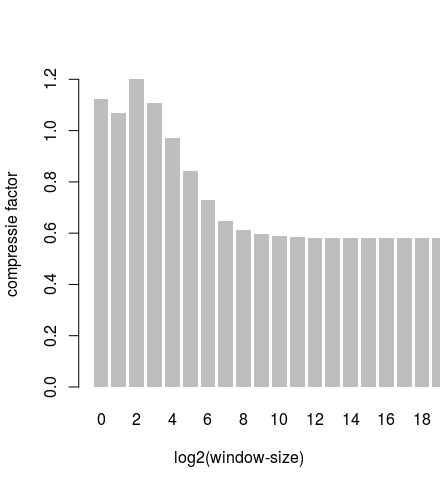
\includegraphics[width=7cm]{images/venstergrootte.png}    
            \end{center}
            \caption{Optimale windowgrootte}
            \label{venstergrootte}
        \end{figure}
    Op deze grafiek valt duidelijk te zien dat vanaf $slidingwindow=2^{12}$ de compressie redelijk constant blijft. Hierdoor kunnen we zeggen dat wanneer de $slidingwindow<2^{12}$ de compressie gemiddeld niet optimaal zal zijn. Dit valt te verklaren doordat er bij kleine window-sizes relatief weinig toppen in een boom zullen zitten.  Deze kunnen dus snel terug uit de boom verwijderd worden. Hierdoor zullen deze misschien later terug opnieuw in de boom moeten gestoken worden met als gevolg dat het volledige karakter samen met het pad van nng opnieuw doorgestuurd zal worden. Bij grotere window-sizes is dit effect veel kleiner. Bij $slidingwindow\geq2^{12}$ kunnen we niet echt een optimale window-grootte bepalen. Bij teksten waarbij er relatief veel lokaliteit\footnote{Met lokaliteit bedoelen we dat in een korte afstand in de tekst bepaalde bytes of sequenties van bytes zich veel herhalen.} is zal een kleinere sliding-window beter presteren dan een grotere. Als er echter weinig lokaliteit aanwezig is, zal een grotere sliding-window de betere optie zijn.
    \subsection{Goede compressie}
     Bij sliding Huffman zal het voorbeeld gegeven bij standaard en adaptive Huffman ook optimaal werken. Er zijn echter nog andere mooie voorbeelden die de voordelen van sliding Huffman aantonen.
     Bijvoorbeeld de string AAAA...BBBB......YYYY...ZZZZ...\label{string-voorbeeld}\footnote{De ... wilt zeggen dat de sequentie voor de punten voor een lange tijd wordt herhaald. } met windowgrootte 2 zal heel dicht bij de compressie van 1 herhaald karakter aanleunen. Dit komt doordat er bijna altijd maar 1 karakter in de boom zal zitten door het verschuiven van de sliding window. 
     Het is eenvoudig in te zien dat standaard Huffman of adaptive Huffman hier veel slechter presteren aangezien deze altijd rekening zullen houden met de andere karakters.
     
        %TODO
%----------------------------------------------------------------------------------------
\section{Two-pass Huffman}

    \subsection{Implementatie}
        Het implementeren van two-pass-Huffman bestaat uit het combineren van verschillende van de 
         reeds besproken algoritmes. Voor het intiële opbouwen van de boom kunnen we het standaard bouw\_boom algoritme \ref{alg:bouwboom} gebruiken.  Om verder de frequenties van de boom dynamisch
         te verlagen gebruiken we algoritme 
         \ref{alg:verlaagfrequentie}: verlaag frequentie. 
        Aangezien er in deze boom geen nng aanwezig zal zijn, gaat het probleem dat zich voor deed
         bij Figuur \ref{fig:verwijderverkeerd} hier niet voorkomen.
         
    \subsection{Goede compressie}
        Two pass zal net zoals de andere algoritmes goed comprimeren bij standaard voorbeelden zoals het blijven herhalen van 1 karakter. Maar two pass zal het over het algemeen slechter doen. Dit is omdat er een grote kost is die in het begin bij het doorsturen van de boom en de gewichten betaald moet worden.
%----------------------------------------------------------------------------------------
\section{Bloksgewijs adaptieve Huffman}

    \subsection{Implementatie}
    De implementatie van bloksgewijs adaptieve Huffman is bijna helemaal analoog aan adaptieve Huffman. Bij het bloksgewijs adaptief algoritme wordt een counter bijgehouden die de boom en de counter reset elke keer dat een welbepaalde blokgrootte wordt bereikt.
        %TODO
    \subsection{Blokgrootte}
    Bij het bepalen van de blokgrootte wordt op dezelfde manier als bij het bepalen van de sliding-window-grootte gewerkt.
    Grafiek \ref{blokgrootte} toont de compressie per blokgrootte aan.
        \begin{figure}[H]
            \begin{center}                
            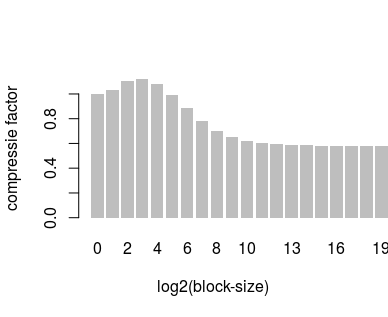
\includegraphics[width=7cm]{images/blokgrootte.png}    
            \end{center}
            \caption{Optimale blokgrootte}
            \label{blokgrootte}

        \end{figure}
    Ook hier kunnen we zien dat bij een blokgrootte van $2^{14}$ de gemiddelde compressie ongeveer constant blijft.
    De slechtere compressie waarbij de $blokgrootte < 2^{14}$ kunnen we wijten aan de kost die we betalen om telkens een boom opnieuw op te bouwen.
    Voor elk nieuw karakter dat toekomt bij de boom moeten we het pad van nng samen met de code van het karakter zelf uitschrijven.
    Bij $blokgrootte \geq 2^{14}$ zal de optimale grootte net zoals bij sliding-window afhangen van de lokaliteit in de tekst. 
    \subsection{Goede compressie}
        %Blokgewijs adaptive Huffman z
        De voorbeelden die goed werken bij sliding window zullen over het algemeen ook goed werken bij blockwise. Indien we dezelfde string AAAA...BBBB......YYYY...ZZZZ... zoals bij sliding gebruiken kunnen we ook een zeer goede compressie bekomen wanneer we de blokgrootte zo groot maken als het aantal keer dat 1 karakter achter elkaar herhaald wordt.


%----------------------------------------------------------------------------------------
\section{Resultaten en vergelijking} \label{1}
    \subsection{Compressie} \label{2}
        \subsubsection{Normale tekst} \label{3}
            Figuur \ref{compressie1} toont de gemiddelde compressie over 50 willekeurige tekst bestanden.
            \begin{figure}[H]
                \begin{center}
                    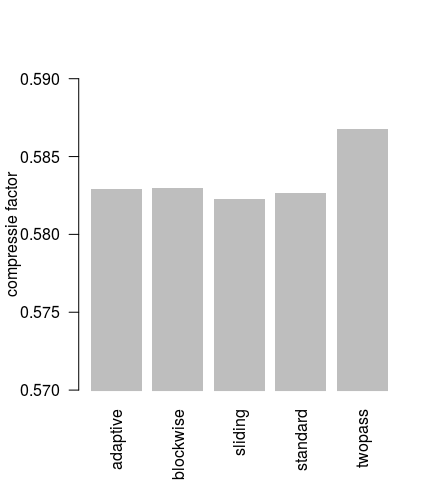
\includegraphics[width=8cm]{images/compressie-tekst.png}    
                \end{center}
                \caption{Gemiddelde compressie normale tekst}
                \label{compressie1}

            \end{figure}
            Hieruit kunnen we duidelijk afleiden dat twopass veruit het slechtste presteert.
            Dit valt te wijten aan de gewichten die in het begin samen met de boom moeten doorgestuurd worden. Deze nemen per blad in de boom 4 tot 8 bytes in beslag. Verder is het voordeel dat we halen uit het verwijderen van frequenties van de karakters die al gepasseerd zijn niet voldoende om de initiële kost van de gewichten te kunnen rechtvaardigen. Een oplossing hiervoor zou het apart encoderen van de gewichten zijn. Hierdoor wordt hun impact geminimaliseerd.
            Verder valt ook op dat de compressiefactor\footnote{$Compressiefactor=nieuwegrootte/orginele grootte$} van standaard-, adaptive- en blokwise-Huffman zeer dicht bij elkaar in de buurt liggen.
            Dit komt overeen met de verwachtingen aangezien standaard Huffman in het begin de hele boom moet doorstuuren, terwijl bij adaptive Huffman de paden en codes online worden doorgestuurd. Deze 2de manier is iets langer doordat de paden samen langer zijn dan de boom. Dit wordt echter gecompenseerd doordat de initiële boom van adaptive leeg is en deze codes zullen in het begin dus korter zijn dan deze van de standaard boom. 
            Blockwise Huffman zal door de grote gelijkenissen met Adaptive Huffman ook sterk in de buurt van deze 2 liggen. Enkel indien er opmerkelijke verschillen zijn tussen de blokken van blockwise zal deze beter encoderen. In de andere gevallen zal de compressiefactor van dit algoritme iets slechter zijn. Als laatste zien we dat sliding-window de beste compressiefactor heeft. Dit komt omdat hij voordeel haalt uit de lokaliteit van de teksten als er bijvoorbeeld een woord voorkomt ergens in het begin van de tekst, is de kans groter dat deze ergens in deze buurt herhaald zal worden.
        \subsubsection{Willekeurige data}
           Figuur \ref{compressie} toont de gemiddelde compressie over 50 willekeurige binaire bestanden.
            
            \begin{figure}[H]
                \begin{center}
                     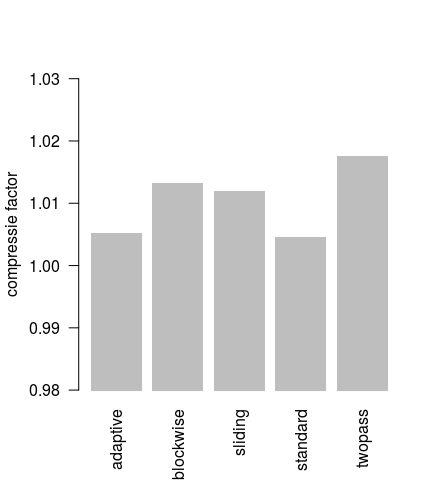
\includegraphics[width=8cm]{images/compressie-random.png}    
                \end{center}
                \caption{Gemiddelde compressie willekeurige data}
                \label{compressie}
            \end{figure}
            Deze figuur demonstreert dat de compressiefactor op willekeurige data overal iets boven de 1 zal liggen. Dit is wederom makkelijk in te zien. De frequenties van alle mogelijke bytes zullen ongeveer evenveel voorkomen. Hierdoor zullen de codeeralgoritmes een boom opstellen die min of meer gebalanceerd is met een diepte 8. Dit wil zeggen dat er een afbeelding van 1 byte op 1 byte ontstaat waardoor er geen compressie gebeurt en we enkel de overhead nog moeten meetellen van de boom of paden van nng die moeten doorgestuurd worden. Deze overhead is het grootst in two-pass doordat de gewichten die door moeten gestuurd worden relatief veel bytes in beslag nemen zeker wanneer bijna elke byte gebruikt zal worden. Na two-pass zijn blockwise en sliding de slechtste. Dit kunnen we verklaren doordat er totaal geen lokaliteit zit in willekeurige data zit. De mechanismes die normaal beter werken bij teksten met veel lokaliteit, worden nu als het ware tegen de algoritmen gebruikt. Standaard en Adaptive zitten wederom zeer dicht bij elkaar. Dit kunnen we op dezelfde manier verklaren als de compressie met gewone tekst gegeven in de voorgaande paragraaf \ref{1} \ref{2} \ref{3}.  
    
            
    \subsection{Snelheid}
        \subsubsection{Encoder}
            \begin{figure}[H]
                \begin{center}
                     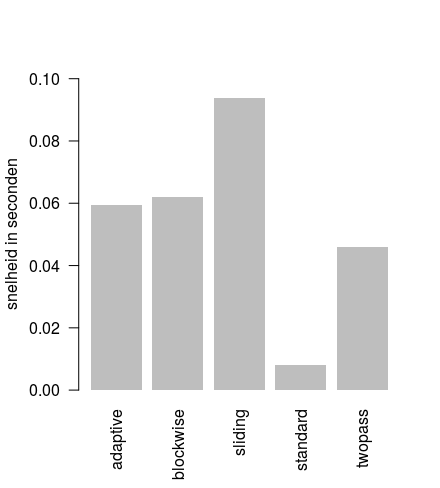
\includegraphics[width=7cm]{images/snelheid-tekst.png}    
                \end{center}
                \caption{Gemiddelde Snelheid encoders}
                \label{compressie-vgl}
            \end{figure}
        
        Figuur \ref{compressie-vgl} toont aan dat standaard Huffman veruit de snelste is. Dit komt doordat er veel meer optimalisatiemogelijkheden zijn. Doordat de boom niet veranderd kan er gemakkelijker aan preprocessing gedaan worden.
        Daarna volgt het two-pass algoritme. Dit algoritme is sneller omdat het reeds op voorhand het bestand in het geheugen laad. De andere algoritme laten dit door hun online aard niet toe. Adaptive en blockwise zijn opnieuw ongeveer even snel aangezien 99 percent van de code hetzelfde is. Het kleine verschil dat aanwezig is, is te wijten aan het steeds heropbouwen van een nieuwe boom bij blockwise nadat de blokgrootte bereikt is. Het traagste algoritme is het sliding-window algoritme. De vertraging ontstaat bij het encoderen waarbij zowel de verhoog\_frequent als de verlaag\_frequentie operaties moeten uitgevoerd worden.
        \subsubsection{Decoder}
            \begin{figure}[H]
                \begin{center}
                 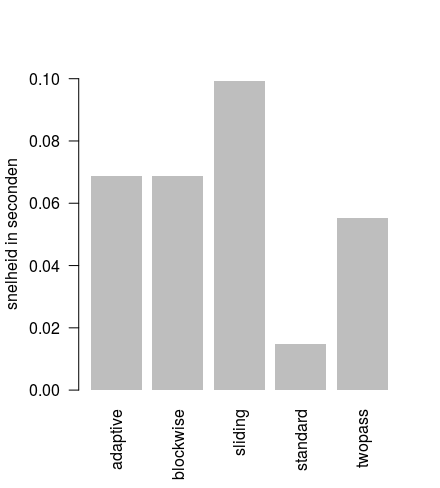
\includegraphics[width=7cm]{images/decodeer-snelheid-tekst.png}    
                \end{center}
                \caption{Gemiddelde Snelheid decoders}
                \label{decoder}
            \end{figure}
        Ook de decodeersnelheid is van groot belang. Decoderen is namelijk over het algemeen meer nodig dan encoderen. Bijvoorbeeld als een bestand geëncodeerd wordt en online ter beschikking wordt gesteld dan moet dit bestand maar 1 keer worden geëncodeerd en kan door meerdere personen gedownload en gedecodeerd worden.
        %over het algemeen veel vaker nodig dan encoderen
        De vergelijking van Figuur \ref{compressie-vgl} met Figuur \ref{decoder} toont aan dat decoderen eenzelfde trend volgt als het encoderen. Opnieuw is standaard Huffman het snelst gevolgd door twopass, adaptive, blockwise en sliding window komt weer binnen als laatste.
    Decoderen is echter steeds een beetje trager dan het encoderen.
        

\section{Bespreking} 
% je zegt hier niets over decompressie? 
%nadelen en voordelen bespreken van elke compressie algoritme
%voorstel bloksgewijs standaard huffman
%decompressie eigenlijk belangrijker

Uit de resultaten van de vorige paragraaf kan afgeleid worden dat de compressie van standaard Huffman en adaptieve Huffman dicht bij elkaar liggen. De keuze tussen adaptive- en standaard Huffman kunnen we dus tot de volgende vraag herleiden: "Moeten de data online gecodeerd worden of niet?". Indien de data niet online gecodeerd moeten worden is standaard Huffman de beste optie. Zowel decoderen als encoderen voert deze variant veel sneller uit dan de andere algoritmes. Wanneer er echter nood is aan een online compressie algoritme is de adaptieve variant aangewezen. Verder is het belangrijk in te zien dat voor gewone tekst de sliding window doorgaans zeer goed presteert, beter zelfs dan standaard en adaptieve Huffman. Maar hiervoor moet je betalen met een langere encodeer en decodeer tijd. Blockwise en twopass slagen er in de praktijk niet in de vergelijking met de alternatieven te doorstaan. Een nadeel van het standaard algoritme is dat online en- en decodering niet mogelijk is. Standaard blockwise Huffman, waarbij standaard Huffman wordt toegepast op blokken van de tekst, biedt hier een oplossing. 
Verder valt ook te zien dat decompressie altijd iets langer duurt dan compressie. Dit is echter ongelukkig want decompressie zal vaker toegepast worden dan compressie.

 

%----------------------------------------------------------------------------------------
\section{Conclusie}
Bij het kiezen van een compressiealgoritmen moeten we verschillende aspecten afwegen: snelheid van het algoritme, nood aan online en- of decodering en aanwezigheid van lokaliteit in de data. Naargelang de vereisten en data wordt een gepast algoritme geselecteerd. Doorgaans is standaard Huffman zeer snel in vergelijking met de andere algoritmes. Het sliding window algoritme comprimeert zeer goed op normale tekst bestanden. Om de voordelen van de verschillende algoritmes te combineren wordt het standaard blockwise Huffman algoritme voorgesteld dat zowel adaptief is, snel is en gebruik maakt van lokaliteit. 
%herhaal de conclusies wat


%----------------------------------------------------------------------------------------
%	REFERENCE LIST
%----------------------------------------------------------------------------------------
\printbibliography
%----------------------------------------------------------------------------------------
\end{document}
